%%%%%%%%%%%%%%%%%%%%%%%%%%%%%%%%%%%%%%%%%%%%%%%%%
%%%
%%% Auteur : Stéphane Péchard - stephane.pechard@univ-nantes.fr
%%% Fichier : introduction.tex - introduction générale de la thèse
%%% Version : 0.1
%%% Date : 2007/11/26
%%%
%%%%%%%%%%%%%%%%%%%%%%%%%%%%%%%%%%%%%%%%%%%%%%%%%

% commandes utiles dans ce chapitre
\newcommand\offset{\mathit{decalage}}
\newcommand\slope{\mathit{pente}}

\chapter[Critère objectif de qualité vidéo fondé sur le débit et une analyse du contenu]{Critère objectif de qualité vidéo \\fondé sur le débit et une analyse du contenu} \label{chap:MQV1}
\opt{final}{\lettrine[lines=4]{N}{ous avons constaté}}\opt{nofinal}{Nous avons constaté} que certains critères objectifs n'étaient pas aussi performants pour la prédiction de la qualité de la TVHD que pour celle de la TVSD. L'objet de ce chapitre est de proposer un critère objectif de qualité vidéo avec référence complète plus adapté au format haute définition. De plus, nous nous situons toujours dans le cadre d'un codage \avc. Dans ce contexte spécifique, nous cherchons à atteindre des performances de prédiction supérieures à celles obtenues par des critères tels que VSSIM et VQM.

Nous savons que pour un même débit, deux séquences de contenu différent peuvent être évaluées de manière très différente par les observateurs. L'un des objectifs de notre critère est donc de caractériser la qualité d'un contenu afin de la distinguer de celle d'un contenu différent. Par ailleurs, pour avoir utiliser le critère de qualité VQM avec les séquences dont nous disposons, nous avons constaté sa complexité calculatoire dans un contexte d'évaluation de la qualité de séquences de TVHD. L'autre objectif du critère proposé est une obtention rapide du résultat. Précisons néanmoins que notre but ici n'est pas de proposer une mise en \oe uvre temps-réel. Nous nous bornerons à montrer la faisabilité et les performances du critère en termes de prédictibilité de la qualité visuelle.

Nous commencerons ce chapitre par décrire le fonctionnement du critère proposé. Puis, nous détaillerons ses différentes conditions d'évaluation et les modèles de prédiction des paramètres du modèle de qualité proposés. Nous terminerons en présentant les performances obtenues sur la base de séquences TVHD dont nous disposons et en les comparant avec celles de VQM et VSSIM.


\section{Description du critère}
La construction du critère découle de l'observation des résultats des évaluations visuelles de qualité. Elle est présentée dans cette première section, le modèle de qualité vidéo y étant décrit. Les paramètres optimaux du modèle seront ensuite déterminés. Nous en déduirons l'impact de la modélisation sur la prédiction.

\subsection{Aspects globaux du critère}
La figure~\ref{fig:schemaMetrique1} présente le schéma global du critère objectif de qualité visuelle proposé. Ce critère est basé sur une analyse spatio-temporelle du contenu qui permet de calculer des paramètres pour chaque séquence. Ces paramètres sont ensuite utilisés pour prédire les deux paramètres $\offset{}$ et $\slope{}$ d'un modèle de qualité vidéo. Ce modèle enfin fournit une prédiction de la qualité de la séquence dégradée. L'évolution de la qualité pour un même contenu à différents débits est simplement déduit par la variation du débit. Ce couplage débit-paramètres permet de prédire l'évolution de la qualité de différents contenus à différents débits de codage. Nous nous distinguons ainsi de la technique d'Oelbaum~\cite{oelbaum-pcs2007} qui calcule des paramètres intra-contenu uniquement. Le point commun entre les deux méthodes est la spécificité à un système dégradant donné.

\begin{figure}[htbp]
\centering
\begin{tikzpicture}[node distance = 3.5cm, auto, text centered]% schéma global de la métrique de qualité vidéo avec référence réduite basée sur la répartition du débit

% \begin{tikzpicture}[node distance = 3.5cm, auto]
% Place nodes
	\node[text width=5em] (seqRef) {séquence de référence};
	\node[action, right of=seqRef, text width=3cm] (classif) {analyse spatio-temporelle du contenu};
	\node[action, right of=classif, text width=2.5cm, node distance = 5cm] (combi) {prédiction des paramètres du modèle};
	\node[below of=seqRef, node distance = 3cm, text width=5em] (belowRef) {séquence dégradée};
	\node[below of=classif, node distance = 3cm] (belowExtract) {};
	\node[action, right of=belowExtract, text width=5em, node distance = 5cm] (modele) {modèle de qualité};
	\node[text width=5em, right of=modele] (mos) {note objective de qualité $Q$};
% Draw edges
	\path[fleche] (seqRef) -- (classif);
	\path[fleche] (classif) -- (combi) node[pos=0.5] {$P_i^S, M^S$};
	\path[fleche] (combi) -- (modele) node[pos=0.5,right] {$\offset, \slope$};
	\path[fleche] (belowRef) -- (modele) node[pos=0.5] {débit $B$};
	\path[fleche] (modele) -- (mos);
% \end{tikzpicture}
\end{tikzpicture}
\caption{Schéma global du critère proposé.}
\label{fig:schemaMetrique1}
\end{figure}


\subsubsection{Analyse spatio-temporelle du contenu}
L'analyse spatio-temporelle du contenu utilisée est celle présentée au chapitre~\ref{chap:methode}. Pour chaque séquence $S$, elle produit les proportions $P_i(S)$ des cinq classes de type de tube spatio-temporel $C_i$ avec $i\in [\text{1};\text{5}]$. Pour chaque tube $t_S$ de chaque séquence $S$, elle fournit les composantes horizontale $M_h(t_S)$ et verticale $M_v(t_S)$ du vecteur de mouvement $M(t_S)$. Le module moyen $M^S$ du mouvement de la séquence $S$ est calculé comme la moyenne des modules des vecteurs de l'ensemble ou d'une sous-partie des $N_t$ tubes de la séquence :
\begin{equation}
M^S = \frac{\lambda}{N_t}\times\sum\limits_{t_S=1}^{N_t} \left(\sqrt{M_h(t_S)^2 + M_v(t_S)^2}\right). \label{eq:mvtTousTubes}
\end{equation}
%
Rappelons que le vecteur de mouvement est calculé à partir du bloc central du tube et que les tubes sont constitués de cinq blocs successifs. Il correspond à une durée de 80 ms comme le montre la figure~\ref{fig:dureeTube}. Les déplacements $M_h(t_S)$ et $M_v(t_S)$ sont ainsi mesurés entre deux images. Ceci explique le facteur $\lambda$ utilisé pour exprimer $M^S$ en pixels par seconde. Dans le cas d'une séquence à 50 trames par secondes, nous avons $\lambda$ = 12,5.

\begin{figure}[htbp]
	\centering
	\begin{tikzpicture}[scale=0.6]
		% schéma du tube dans une image

\draw[help lines, dashed] (1.1,-3) -- (21.8,-3);
\draw[help lines, dashed] (2.1,-2.5) -- (22.9,-2.5);
\draw[help lines, dashed] (2.1,-1) -- (22.9,-1);

\filldraw[help lines, fill=blue!20] (1.1,-3) -- (2.1,-2.5) --  (2.1,-1) -- (1.1,-1.5) -- cycle;
\filldraw[help lines, fill=blue!20] (6.3,-3) -- (7.3,-2.5) --  (7.3,-1) -- (6.3,-1.5) -- cycle;
\fill[fill=blue!20] (11.5,-3) -- (12.5,-2.5) --  (12.5,-1) -- (11.5,-1.5) -- cycle;
\filldraw[help lines, fill=blue!20] (16.7,-3) -- (17.7,-2.5) --  (17.7,-1) -- (16.7,-1.5) -- cycle;
\filldraw[help lines, fill=blue!20] (21.9,-3) -- (22.9,-2.5) --  (22.9,-1) -- (21.9,-1.5) -- cycle;

\draw[help lines, dashed] (1.1,-1.5) -- (21.9,-1.5);


% \begin{tikzpicture}[scale=0.5]
\foreach \i in {0.25,0.75,1.25,1.75} % grille sur l'image centrale
{
	\draw (10+2*\i,\i) -- (10+2*\i,-6+\i);
	\draw (10,-3*\i) -- (14,2-3*\i);

	\foreach \j in {0,1,3,4} % grille sur les autres images
	{
		\draw (5*\j + 2*\i, \i) -- (5*\j + 2*\i, -6 + \i);
		\draw (5*\j,-3*\i) -- (5*\j + 4,2-3*\i);
	}
}

\draw (2,-6.5) node{$i-2$};
\draw (7,-6.5) node{$i-1$};
\draw (12,-6.5) node{image $i$};
\draw (17,-6.5) node{$i+1$};
\draw (22,-6.5) node{$i+2$};

\draw[<->] (12,2) -- (22,2) node[above,pos=0.5] {80 ms};
\draw[<->] (2,3) -- (22,3) node[above,pos=0.5] {tube};

% \end{tikzpicture}

	\end{tikzpicture}
	\caption{Exemple de tube avec la durée correspondant au vecteur de mouvement.}
  \label{fig:dureeTube}
\end{figure}

Les proportions des classes de contenu correspondent à celles calculées sur une séquence comme nous l'avons fait à la section~\ref{sec:methodeClassifST}. Le tableau~\ref{tab:proportionsClasses} de la page~\pageref{tab:proportionsClasses} présente les proportions des douze séquences de la sous-base SVT2006, après suppression des zones sans classes et des ambiguïtés de classification. Le tableau~\ref{tab:proportionsClassesSVTEuro} présente celles des douze autres séquences de la base.

\begin{table}[htbp]
\centering
\begin{tabular}{cccccc}\toprule
\strong{contenu}						& $C_1$ 		& $C_2$		& $C_3$ 		& $C_4$		& $C_5$ 	\\ \toprule
\emph{New Mobile \& Calendar}	& 5,59			& 42,64		& 20,59		& 23,47		& 7,71		\\ \midrule
\emph{Parkrun}							& 0,34			& 17,58		& 19,90		& 40,19		& 21,99		\\ \midrule
\emph{Knightshields}					& 12,13		& 39,50		& 27,05  		& 12,88		&	 8,44		\\ \midrule
\emph{Stockholm Pan}				& 2,39			& 47,06 		& 20,61 		&	8,51 		& 21,43		\\ \midrule
\emph{Concert}							& 39,39		& 47,05  		& 9,35  		& 1,20  		& 3,01		\\ \midrule
\emph{Foot }								& 0,03			& 62,84		& 13,27  		& 9,53 			& 14,33 	\\ \midrule
\emph{Movie}								& 8,77			& 70,47 		& 13,44  		& 5,73  		& 1,59		\\ \midrule
\emph{Voile}								& 0,84			& 86,26  		& 8,22  		& 0,54 			& 4,14		\\ \midrule
\emph{Credits}							& 36,27		& 23,10  		& 13,91  		& 20,89   		& 5,83		\\ \midrule
\emph{Golf}									& 2,49			& 69,11		& 19,81  		& 1,48  		& 7,11		\\ \midrule
\emph{Show}								& 36,13		& 39,69		& 14,72  		& 2,17  		& 7,29		\\ \midrule
\emph{Standing}							& 81,64		& 2,85			& 11,30  		& 0,62			& 3,59 		\\ \bottomrule
\end{tabular}
\caption{Proportions, exprimées en pourcentage, des classes des contenus des sous-bases Euro1080 et SVT2002.}
\label{tab:proportionsClassesSVTEuro}
\end{table}


\subsubsection{Prédiction des paramètres du modèle de qualité}
La prédiction des paramètres du modèle de qualité est une étape critique car elle fournit à ce modèle les résultats de l'analyse spatio-temporelle du contenu. Nous détaillerons cette prédiction à la section suivante.


\subsubsection{Codage}
Les séquences dégradées sont celles présentées à l'annexe~\ref{annex:base}. Elles sont produites par un codage \avc{} réalisé avec le codeur de référence~\cite{h264-jm}. Le débit $B$, supposé connu, correspond à celui utilisé par ce codeur. Les sept débits des 24 contenus sont donnés dans le tableau~\ref{tab:bitratesHD} de la page~\pageref{tab:bitratesHD}.


\subsubsection{En sortie du modèle}
Le modèle de qualité proposé ne fournit pas directement une prédiction du MOS mais une prédiction de la différence de qualité entre la séquence de référence cachée et la séquence dégradée, c'est-à-dire DMOS($S_j,B_k$) = MOS($S_j$) - MOS($S_j,B_k$). Cette manière de procéder est classique pour un critère avec référence complète. En fait, afin d'utiliser un modèle de qualité croissant avec le débit, nous considérons ici la valeur 100 $-$ DMOS($S_j,B_k$). Nous posons donc :
\begin{equation}
Q(S_j,B_k) = \text{100} - \text{DMOSp}(S_j,B_k).
\end{equation}
%
Ainsi, le critère de qualité sera évalué en comparant les valeurs 100 $-$ DMOS($S_j,B_k$) aux $Q(S_j,B_k)$ issus du modèle et auxquels une fonction d'ajustement est appliquée. Afin de distinguer les valeurs 100 $-$ DMOS($S_j,B_k$) des DMOS, nous les appellerons \Dcent{} dans la suite de ce chapitre.


\subsection{Modèle de qualité vidéo}
Le modèle proposé est basé sur les résultats de l'évaluation subjective de la qualité vidéo des séquences de la base présentée à l'annexe~\ref{annex:base}. La figure~\ref{fig:DMOSrateCodeurRefHD} présente quelques exemples de \Dcent{} en fonction du débit. Hormis quelques irrégularités imputables au codeur, ces \Dcent{} suivent une tendance commune. La croissance est rapide à bas débit et plus lente à partir d'un débit donné. De plus, dans un contexte de télévision haute définition, nous cherchons une bonne modélisation pour les qualités moyennes et hautes, c'est-à-dire au moins supérieures à 40. Il n'est donc pas nécessaire d'être particulièrement précis en dessous de cette valeur. Ceci est cohérent avec les mesures subjectives de notre base, où la majorité des évaluations sont supérieures à ce seuil. Nous proposons un modèle général de la qualité $Q$ d'une séquence vidéo en fonction du débit de codage $B$ de la forme :
\begin{equation}
Q = L \left(1 - e^{-\frac{B - \offset}{\slope}}\right)
\end{equation}
%
avec $L$ limite asymptotique vers laquelle $Q$ tend lorsque $B$ augmente et $\offset$ et $\slope$ les deux paramètres du modèle de qualité.

\begin{figure}[htbp]
\centering
\subfloat{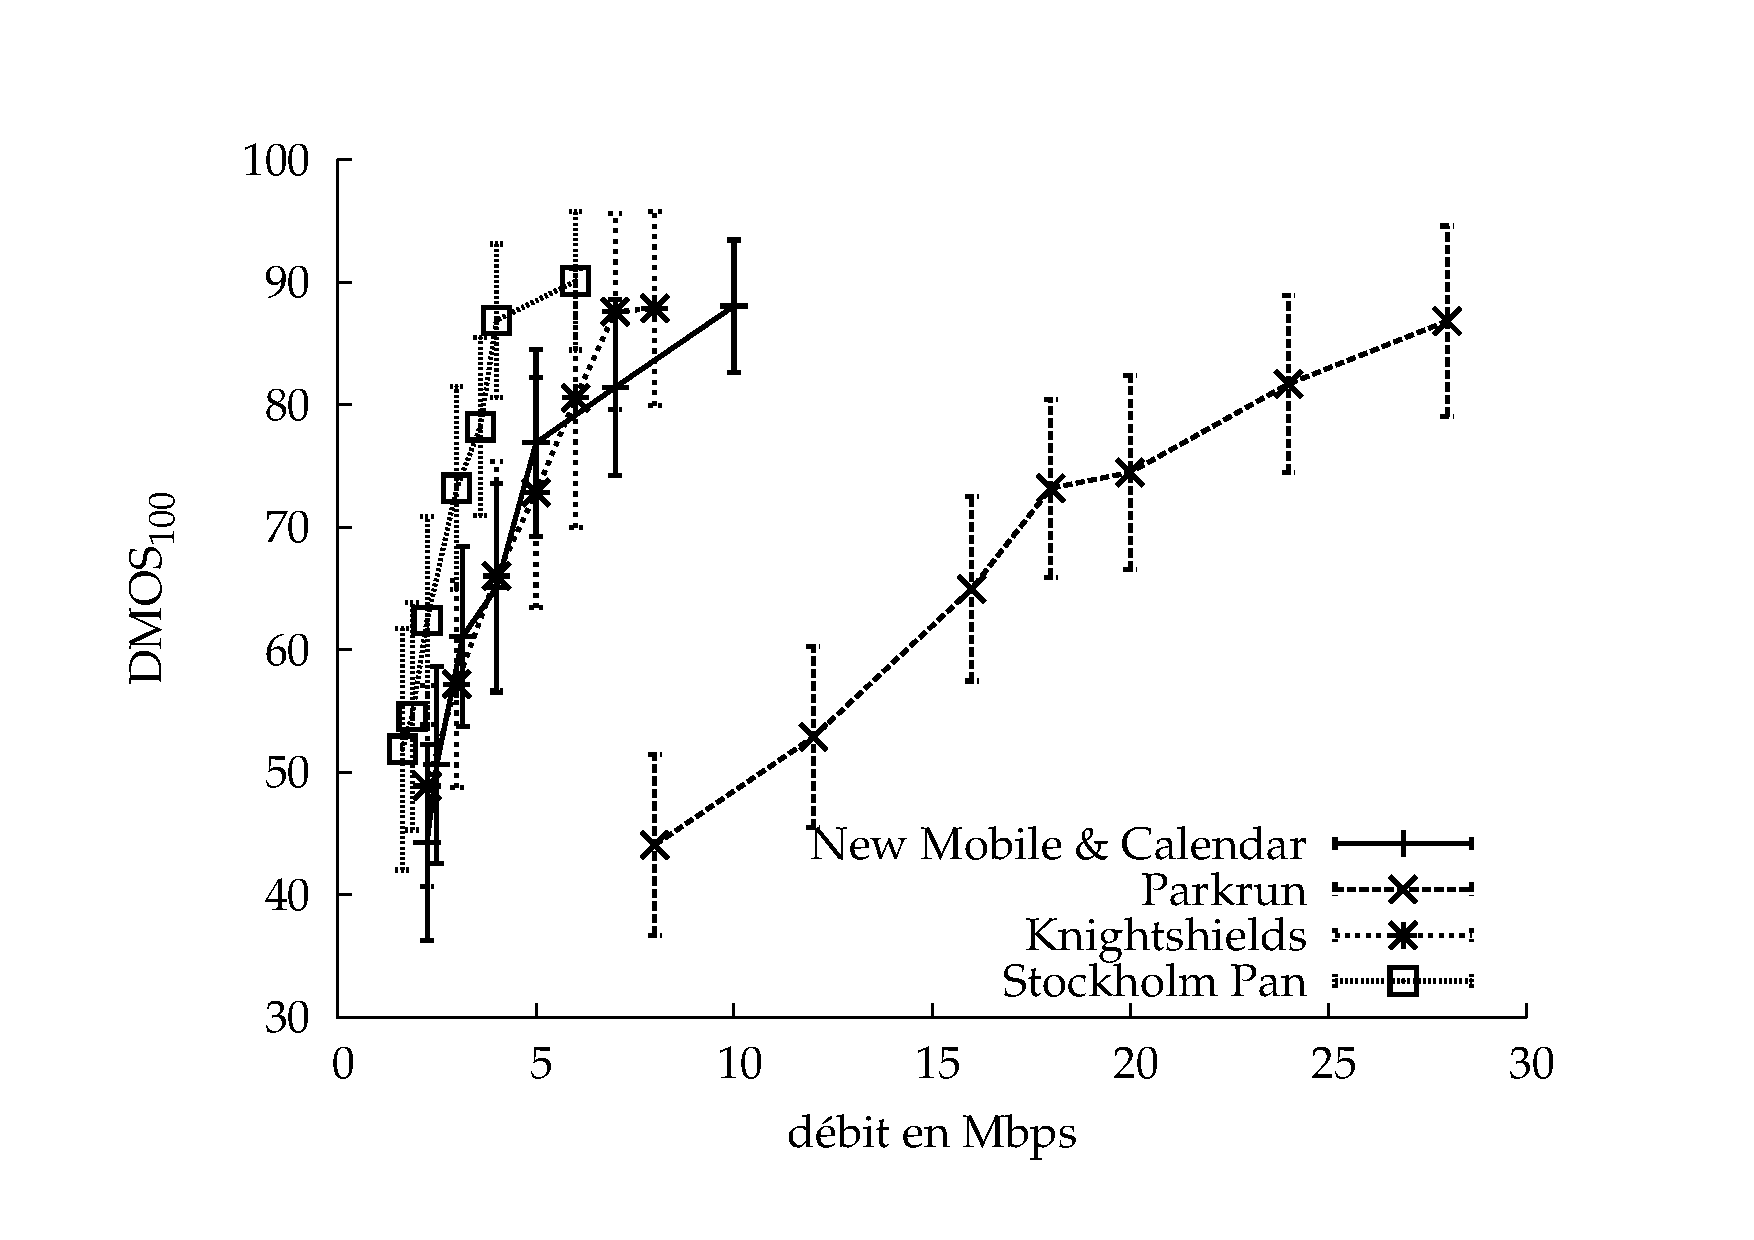
\includegraphics[page=1, width=0.49\linewidth, trim= 70 50 90 70]{plot/chap7/svtEuro1080-2-DMOS100.pdf}}\hfill
\subfloat{\includegraphics[page=2, width=0.49\linewidth, trim= 70 50 90 70]{plot/chap7/svtEuro1080-2-DMOS100.pdf}}\\
\caption{\Dcent{} en fonction du débit, exprimé en Mbps, pour huit contenus.}
\label{fig:DMOSrateCodeurRefHD}
\end{figure}

Les paramètres $\offset$ et $\slope$ permettent de distinguer les contenus les uns des autres, ils correspondent aux différences inter-contenus. Le débit est utilisé pour distinguer les séquences dégradées correspondant à un contenu donné. Il est déterminé par le codage H.264 effectué, alors que les paramètres $\offset$ et $\slope$ le sont à partir du mouvement moyen et des proportions de chaque classe de contenu présente dans la séquence. $\offset$ correspond au débit pour lequel $Q$ = 0, c'est-à-dire au décalage à l'origine du modèle. Ce paramètre permet d'ajuster cette origine en fonction des basses qualités. Il s'exprime en Mbps. $\slope$ correspond à la pente du modèle. Plus il est faible, plus le modèle croit rapidement. Il est de dimension inverse au débit, il s'exprime donc en Mbps$^{-1}$.

L'évaluation de qualité effectuée sur la base présentée à l'annexe~\ref{annex:base} génère des notes de qualité allant de 0 à 100. Notre critère doit donc produire des notes dans cet intervalle, même si cette valeur théorique n'est pas atteinte en pratique. C'est pourquoi nous fixons $L=100$, d'où :
\begin{equation}
Q = 100 \left(1 - e^{-\frac{D - \offset}{\slope}}\right) \label{eq:modele}.
\end{equation}
%
C'est cette forme qui sera utilisée dans la suite de ce chapitre.

D'autres modèles ont été évalués, comme par exemple des modèles polynomiaux ou logistique. Le modèle retenu est celui minimisant la perte de précision due à son utilisation avec des paramètres optimaux que nous explicitons maintenant.


\subsection{Paramètres optimaux du modèle}
Le modèle utilise deux paramètres par contenu. Pour chaque contenu, nous pouvons déterminer quelles valeurs de ces paramètres permettent de s'approcher au plus près du jugement humain, c'est-à-dire des \Dcent.  C'est ce que nous appelons les paramètres optimaux, notés $\offset^{\textit{opt}}$ et $\slope^{\textit{opt}}$. Nous les calculons en ajustant le modèle de qualité aux \Dcent. Les valeurs obtenues sont présentées dans le tableau~\ref{tab:paramNomin}.

\begin{table}[htbp]
\centering
\begin{tabular}{ccccccc}\toprule
\textbf{contenu}							& $\offset^{\textit{opt}}$	& $\slope^{\textit{opt}}$	& & \textbf{contenu}						& $\offset^{\textit{opt}}$	& $\slope^{\textit{opt}}$\\ \toprule
\multirow{2}{2.4cm}{\emph{New Mobile \& Calendar}}& \multirow{2}{1.1cm}{-0,4243}  	&  \multirow{2}{1.1cm}{4,1515} 	& & \multirow{2}{3cm}{\emph{Above Marathon}}			& \multirow{2}{1.1cm}{1,1793}   							& \multirow{2}{1.2cm}{13,8381} \\
& \\\midrule
\emph{Parkrun}					& 0,1923 		&  14,3482 	& & \emph{Captain}						& -0,4923  							& 4,5618 \\ \midrule
\emph{Knightshields}			& -0,2792  	&  3,8581 	& & \emph{Dance in the Woods}	& 0,2007   							& 6,4184\\ \midrule
\emph{Stockholm Pan}		& 0,0239  	&  2,2578 	& & \emph{Duck Fly}						& -2,3363  							& 16,2053\\ \midrule
\emph{Concert}					& -10,0858 	&  18,0244 	& & \emph{Fountain Man}				& -2,1401 							& 11,6200\\ \midrule
\emph{Foot}						& -3,7233 	&  11,7979 	& & \emph{Group Disorder}			& -0,9410    							& 8,3570\\ \midrule
\emph{Movie}						& -1,9514  	&  7,1616 	& & \emph{Inside Marathon}			& -2,0182    							& 9,3178\\ \midrule
\emph{Voile}						& -0,2859  	&  5,7236 	& & \emph{New Parkrun}				& -2,8826    							& 7,4945\\ \midrule
\emph{Crédits}					& -0,0096  	&  6,5395 	& & \emph{Rendezvous}					&  0,1118   							& 13,7035\\ \midrule
\emph{Golf}							& -0,3152  	&  2,4658 	& & \emph{Stockholm Travel}			& -2,9660    							& 6,1537\\ \midrule
\emph{Show}						& -2,3570  	&  5,8756 	& & \emph{Tree Pan}						& -0,2026    							& 2,6155\\\midrule
\emph{Standing}					& -1,3161  	&  2,4832 	& & \emph{Ulriksdals}						& -2,9860    							& 9,1737\\ \bottomrule
\end{tabular}
\caption{Paramètres optimaux du modèle de qualité pour chaque contenu.}
\label{tab:paramNomin}
\end{table}

Les valeurs de $\offset^{\textit{opt}}$ sont majoritairement proches de zéro. Cela signifie que le décalage à l'origine est globalement faible. Quelques séquences se distinguent néanmoins, et notamment \emph{Concert} avec $\offset^{\textit{opt}}$ = -10,0858. Une telle valeur négative signifie que le contenu atteint de bonnes qualités avec un débit relativement faible. Notons cependant que l'exemple du contenu \emph{Concert} est sans doute extrême du fait de sa non-monotonie, observable figure~\ref{fig:MOSrateCodeurRefHD} de la page~\pageref{fig:MOSrateCodeurRefHD}, ce qui peut expliquer les deux valeurs marginales de $\offset^{\textit{opt}}$ et $\slope^{\textit{opt}}$ pour cette séquence. Le reste des valeurs est compris entre -3,7 et 1,2. Les valeurs de $\slope^{\textit{opt}}$ vont de 2,2578 à 18,0244. Les plus fortes valeurs correspondent aux séquences les plus complexes comme \emph{Parkrun}, \emph{Above Marathon}, \emph{Duck Fly} ou \emph{Rendezvous}. Cela est logique dans la mesure où la croissance de la qualité d'une séquence complexe est plus lente que celle d'une séquence simple. En effet, une séquence complexe a besoin d'un incrément de débit plus important pour gagner autant en qualité qu'une séquence de complexité moindre. Ainsi, les faibles valeurs de $\slope^{\textit{opt}}$ correspondent aux séquences \emph{Stockholm Pan}, \emph{Golf}, \emph{Standing} ou \emph{Tree Pan}. Cet ensemble de valeurs représente ce que doit fournir l'étape de prédiction des paramètres du modèle. Évidemment, les performances du critère de qualité seront mesurées par rapport aux \Dcent{} réels et non en utilisant ces paramètres optimaux.


\subsection{Perte de précision due à la modélisation}
La modélisation n'étant qu'une approximation de la réalité, même les paramètres optimaux ne permettent pas une prédiction parfaite des \Dcent. Un premier indicateur de la capacité du modèle à prédire les \Dcent{} est de l'utiliser avec les paramètres optimaux et de comparer les \Dcent{} prédits de cette manière avec les \Dcent{} réels. Ces \Dcent{} prédits sont nommés \DcentOpt{} et sont obtenus après une fonction d'ajustement. La figure~\ref{fig:MOSpMQV1-MOSLCD} présente les \Dcent{} réels en fonction des \DcentOpt{} pour l'ensemble de 168 séquences dégradées et évaluées sur un écran LCD de la base présentée à l'annexe~\ref{annex:base}. Les indicateurs de performances calculés entre les \Dcent{} et les \DcentOpt{} sont présentés dans le tableau~\ref{tab:perfModOptim}. L'intervalle de confiance sur le coefficient de corrélation (cc) est [0,9730;0,985]. La relation est donc très forte entre les deux ensembles de données, ce que confirme le coefficient de corrélation de rang (ccr). Les deux erreurs (reqm et reqmp) sont très faibles, surtout au regard des intervalles de confiance sur les MOS présentés dans l'annexe~\ref{annex:base}. La perte de précision est donc faible. L'\emph{outlier ratio} (or) confirme ces bonnes performances avec seulement 9,5\% de configurations mal prédites. Ceci nous permet d'envisager l'utilisation du modèle proposé dans notre critère de qualité vidéo.

\begin{table}[htbp]
\centering
\begin{tabular}{ccccc}\toprule
\strong{cc}	& \strong{ccr}	& \strong{reqm} 	& \strong{reqmp}	& \strong{or} 	\\ \toprule
0,9800		& 0,9695		& 3,6591		& 0,5541		& 0,0952		\\ \bottomrule
\end{tabular}
\caption{Performances obtenues par le modèle avec utilisation des paramètres optimaux.}
\label{tab:perfModOptim}
\end{table}

\begin{figure}[htbp]
	\centering
	\begin{tikzpicture}[only marks, scale=0.07]
	\pgfsetplotmarksize{1cm}
	\draw plot[mark=+] file {plot/chap6/MOSpMQV1-MOSLCD.txt};
	\draw[->] (0,0) -- coordinate (x axis) (105,0);
	\draw[->] (0,0) -- coordinate (y axis) (0,105);
	\foreach \x in {0,20,40,60,80,100} \draw (\x cm,1cm) -- (\x cm,-1cm) node[anchor=north] {\x};
	\foreach \y in {0,20,40,60,80,100} \draw (1cm,\y cm) -- (-1cm,\y cm) node[anchor=east] {\y};
	\node[below=0.5cm] at (x axis) {\DcentOpt};
	\node[rotate=90] at (-15,50) {\Dcent};
	\draw[dotted] (0,0) -- (100,100);
	\end{tikzpicture}
	\caption{\Dcent{} des 168 séquences dégradées de la base de l'annexe~\ref{annex:base} en fonction des \DcentOpt{} prédits par le modèle de qualité en utilisant les paramètres optimaux.}
	\label{fig:MOSpMQV1-MOSLCD}
\end{figure}


\section{Prédiction des paramètres du modèle de qualité vidéo}
Les paramètres du modèle sont liées aux différences de qualité observées entre les contenus mais sont indépendants du débit. Nous considérons deux facteurs intrinsèques au contenu influant sur cette différenciation : le mouvement et les proportions respectives des classes de contenu.

Le mouvement intervient à deux niveaux antagonistes. Il est d'abord facteur de surcout pour le codeur, car plus il y a de mouvement, plus les vecteurs de mouvement nécessitent un débit élevé pour être codés. Parallèlement, à partir d'une quantité de mouvement donnée, plus le mouvement d'une zone est important, plus les dégradations de cette zone sont masquées. Cela diminue leur impact sur la perception de la qualité et permet donc de diminuer le débit. Les proportions interviennent en tant qu'indicateurs de la répartition du débit. En effet, à débit constant, une séquence contenant majoritairement des zones homogènes aura tendance à être de qualité supérieure à celle d'une séquence contenant majoritairement des zones de textures.

Pour ces deux facteurs, nous proposons plusieurs contextes de paramétrisation qui permettent d'évaluer le modèle de qualité dans différentes situations. Pour cela, nous exploiterons les données fournies par la classification spatio-temporelle. Dans un second temps, nous proposerons plusieurs modèles de prédiction des paramètres du modèle de qualité vidéo. %Ces modèles de prédiction seront construits à partir des données de mouvement et de proportions.


\subsection{Contextes d'évaluation du modèle}
Nous exploitons de plusieurs manières différentes la classification spatio-temporelle du contenu des séquences. Au total, cela nous fournit quatre contextes d'évaluation du modèle de qualité. Considérons tout d'abord le mouvement moyen de la séquence $S$, nommé $M^S$. Nous l'avons défini à la relation~\ref{eq:mvtTousTubes} comme la moyenne des modules des vecteurs de mouvement de l'ensemble des $N_t$ tubes de la séquence. En fait, nous pouvons restreindre cette définition à un ensemble de tubes plus réduit. En effet, nous considérons que la fiabilité de l'estimation de mouvement effectuée varie selon le contenu. Par exemple, le calcul des vecteurs de mouvement des zones homogènes est moins stable que celui des zones de textures. En fait, cette estimation est d'autant plus stable que l'activité spatio-temporelle du tube est importante. Ceci est illustré figure~\ref{fig:tubeZones}.

\begin{figure}[htbp]
	\centering
	\subfloat[Estimation de mouvement dans une zone homogène. Un décalage de quelques pixels modifie peu l'erreur utilisée pour la sélection du vecteur de mouvement. L'estimation est peu fiable.]{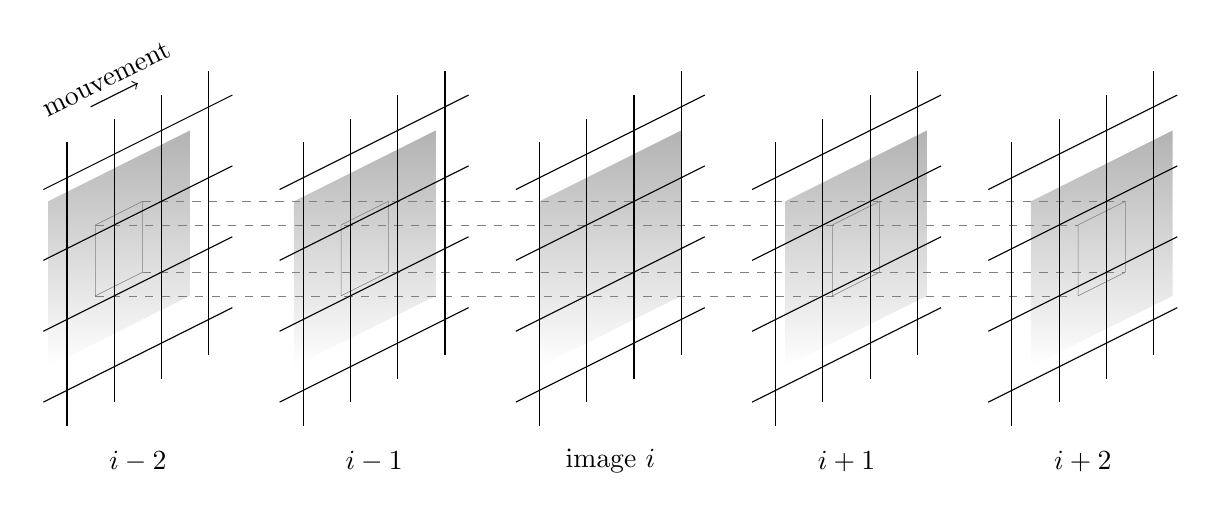
\begin{tikzpicture}[scale=0.6]

\shade[top color=black!30,shading=axis] (0.1,-4.5) -- (3.1,-3) --  (3.1,0.5) -- (0.1,-1) -- cycle;
\shade[top color=black!30,shading=axis] (5.3,-4.5) -- (8.3,-3) --  (8.3,0.5) -- (5.3,-1) -- cycle;
\shade[top color=black!30,shading=axis] (10.5,-4.5) -- (13.5,-3) --  (13.5,0.5) -- (10.5,-1) -- cycle;
\shade[top color=black!30,shading=axis] (15.7,-4.5) -- (18.7,-3) --  (18.7,0.5) -- (15.7,-1) -- cycle;
\shade[top color=black!30,shading=axis] (20.9,-4.5) -- (23.9,-3) --  (23.9,0.5) -- (20.9,-1) -- cycle;

\draw[help lines] (1.1,-3) -- (2.1,-2.5) --  (2.1,-1) -- (1.1,-1.5) -- cycle;
\draw[help lines] (6.3,-3) -- (7.3,-2.5) --  (7.3,-1) -- (6.3,-1.5) -- cycle;
\draw[help lines] (16.7,-3) -- (17.7,-2.5) --  (17.7,-1) -- (16.7,-1.5) -- cycle;
\draw[help lines] (21.9,-3) -- (22.9,-2.5) --  (22.9,-1) -- (21.9,-1.5) -- cycle;

\draw[help lines, dashed] (1.1,-3) -- (21.8,-3);
\draw[help lines, dashed] (2.1,-2.5) -- (22.9,-2.5);
\draw[help lines, dashed] (2.1,-1) -- (22.9,-1);
\draw[help lines, dashed] (1.1,-1.5) -- (21.9,-1.5);

\foreach \i in {0.25,0.75,1.25,1.75} % grille sur l'image centrale
{
	\draw (10+2*\i,\i) -- (10+2*\i,-6+\i);
	\draw (10,-3*\i) -- (14,2-3*\i);

	\foreach \j in {0,1,3,4} % grille sur les autres images
	{
		\draw (5*\j + 2*\i, \i) -- (5*\j + 2*\i, -6 + \i);
		\draw (5*\j,-3*\i) -- (5*\j + 4,2-3*\i);
	}
}

\draw[->] (1,1) -- (2,1.5) node[rotate=26.5,above,pos=0.5] {mouvement};

\draw (2,-6.5) node{$i-2$};
\draw (7,-6.5) node{$i-1$};
\draw (12,-6.5) node{image $i$};
\draw (17,-6.5) node{$i+1$};
\draw (22,-6.5) node{$i+2$};

\end{tikzpicture}
}\\
	\subfloat[Estimation de mouvement dans une zone fortement texturée. Un décalage de quelques pixels modifie fortement l'erreur utilisée pour la sélection du vecteur de mouvement. L'estimation est donc fiable.]{\begin{tikzpicture}[scale=0.59]
\shorthandoff{!} % debug pgf

\draw[draw=white,pattern=crosshatch,pattern color=black!60] (0.1,-4.5) -- (3.1,-3) --  (3.1,0.5) -- (0.1,-1) -- cycle;
\draw[draw=white,pattern=crosshatch,pattern color=black!60] (5.3,-4.5) -- (8.3,-3) --  (8.3,0.5) -- (5.3,-1) -- cycle;
\draw[draw=white,pattern=crosshatch,pattern color=black!60] (10.5,-4.5) -- (13.5,-3) --  (13.5,0.5) -- (10.5,-1) -- cycle;
\draw[draw=white,pattern=crosshatch,pattern color=black!60] (15.7,-4.5) -- (18.7,-3) --  (18.7,0.5) -- (15.7,-1) -- cycle;
\draw[draw=white,pattern=crosshatch,pattern color=black!60] (20.9,-4.5) -- (23.9,-3) --  (23.9,0.5) -- (20.9,-1) -- cycle;

\draw[thick] (1.1,-3) -- (2.1,-2.5) --  (2.1,-1) -- (1.1,-1.5) -- cycle;
\draw[thick] (6.3,-3) -- (7.3,-2.5) --  (7.3,-1) -- (6.3,-1.5) -- cycle;
\draw[thick] (11.5,-3) -- (12.5,-2.5) --  (12.5,-1) -- (11.5,-1.5) -- cycle;
\draw[thick] (16.7,-3) -- (17.7,-2.5) --  (17.7,-1) -- (16.7,-1.5) -- cycle;
\draw[thick] (21.9,-3) -- (22.9,-2.5) --  (22.9,-1) -- (21.9,-1.5) -- cycle;

\draw[thick, dashed] (1.1,-3) -- (21.8,-3);
\draw[thick, dashed] (2.1,-2.5) -- (22.9,-2.5);
\draw[thick, dashed] (2.1,-1) -- (22.9,-1);
\draw[thick, dashed] (1.1,-1.5) -- (21.9,-1.5);

\foreach \i in {0.25,0.75,1.25,1.75} % grille sur l'image centrale
{
	\draw (10+2*\i,\i) -- (10+2*\i,-6+\i);
	\draw (10,-3*\i) -- (14,2-3*\i);

	\foreach \j in {0,1,3,4} % grille sur les autres images
	{
		\draw (5*\j + 2*\i, \i) -- (5*\j + 2*\i, -6 + \i);
		\draw (5*\j,-3*\i) -- (5*\j + 4,2-3*\i);
	}
}

\draw[->] (1,1) -- (2,1.5) node[rotate=26.5,above,pos=0.5] {mouvement};

\draw (2,-6.5) node{$i-2$};
\draw (7,-6.5) node{$i-1$};
\draw (12,-6.5) node{image $i$};
\draw (17,-6.5) node{$i+1$};
\draw (22,-6.5) node{$i+2$};

\shorthandon{!}
\end{tikzpicture}
}
	\caption{Estimation de mouvement dans deux zones d'activité différente. Un décalage de quelques pixels a un impact différent sur l'erreur utilisée pour la sélection du vecteur de mouvement. La fiabilité de l'estimation de mouvement en dépend directement.}
	\label{fig:tubeZones}
\end{figure}

Ainsi, nous définissons deux manières de calculer la grandeur $M^S$. La première est celle de la relation~\ref{eq:mvtTousTubes}. Nous l'appellerons $M^S_1$. La seconde restreint l'ensemble des tubes à ceux appartenant aux classes de forte activité spatio-temporelle, c'est-à-dire les classes de textures moyennes et fortes $C_4$ et de contours $C_5$ :
\begin{equation}
M^S_2 = \frac{\lambda}{N_n^{45}}\times\sum\limits_{t_S=1}^{N_n^{45}} \left(\sqrt{M_h(t_S)^2 + M_v(t_S)^2}\right)
\end{equation}
%
avec $t_S \in [C_4,C_5]$ et $N_n^{45}$ le nombre de tubes des classes de textures moyennes et fortes $C_4$ et de contours $C_5$. La figure~\ref{fig:MVtoutMVC4C5} présente les valeurs de $M^S_2$ en fonction de celles de $M^S_1$ pour les 24 contenus dont nous disposons. Nous remarquons que la majorité des valeurs des deux ensembles sont proches, mais que certaines se distinguent particulièrement. C'est le cas par exemple des séquences \emph{Concert}, \emph{Movie}, \emph{Standing}, \emph{Captain}, \emph{Fountain Man} qui se distinguent par une très faible proportion de textures fortes et de contours. Nous constatons que cela se répercute ici par une faible valeur de $M^S_2$ par rapport à $M^S_1$.

\begin{figure}[htbp] % CC = 0.8895, RMSE = 78.3415
	\centering
	\begin{tikzpicture}[only marks, scale=0.07]
	\pgfsetplotmarksize{1cm}
	\draw plot[mark=+] file {plot/chap6/MVtout-MVC4C5.txt};
	\draw[->] (0,0) -- coordinate (x axis) (85,0);
	\draw[->] (0,0) -- coordinate (y axis) (0,85);
	\foreach \x in {0,20,40,60,80} \draw (\x cm,1cm) -- (\x cm,-1cm);
	\foreach \x in {0,200,400,600,800} \node[anchor=north] at(\x/10,-1) {\x};
	\foreach \y in {0,20,40,60,80} \draw (1cm,\y cm) -- (-1cm,\y cm);
	\foreach \y in {0,200,400,600,800} \node[anchor=east] at(-1,\y/10) {\y};
	\node[below=0.5cm] at (x axis) {$M^S_1$};
	\node[rotate=90] at (-15,42) {$M^S_2$};
	\draw[dotted] (0,0) -- (80,80);
	\end{tikzpicture}
	\caption{Valeurs de $M^S_2$ en fonction de celles de $M^S_1$ en pixels par seconde.}
	\label{fig:MVtoutMVC4C5}
\end{figure}

Les proportions de contenu peuvent également être calculées de deux manières différentes. En effet, rappelons que la segmentation des séquences n'est pas complète. Une technique est utilisée pour attribuer une classe aux pixels des zones vides et des zones avec ambiguïtés de classification dues au mouvement. Ainsi, la somme $\Sigma_p$ des proportions, exprimée en pourcentages, est égale à 100 après l'application de cette technique. Cependant, plus la séquence contient de mouvement, plus les zones non étiquetées peuvent être importantes. Elles sont également plus importantes pour les séquences comportant de grandes zones homogènes, où l'estimation de mouvement sera moins fiable.

Considérer les proportions avant application de l'algorithme est ainsi une manière de tenir compte à la fois du mouvement et des erreurs d'estimation de mouvement. Dans ce cas, la somme des proportions, est inférieure à 100, nous la notons $\Sigma_v$. $\Sigma_p$ et $\Sigma_v$ sont les deux autres contextes d'évaluation du modèle. Les valeurs obtenues sont présentées dans le tableau~\ref{tab:MVC4C5}. La figure~\ref{fig:MVC4C5-SigmaV} présente les valeurs de $\Sigma_v$ en fonction de $M^S_2$ pour les 24 contenus de la base.

\begin{table}[htbp]
\centering
\begin{tabular}{ccp{1cm}cc}\toprule
\textbf{contenu}							& $\Sigma_v$ (\%)	& & \textbf{contenu}						& $\Sigma_v$ (\%)	\\ \toprule
\emph{New Mobile \& Calendar}	& 97,1915 		& & \emph{Above Marathon}			& 95,8314 		\\ \midrule
\emph{Parkrun}							& 97,6503 		& & \emph{Captain}						& 84,0237 		\\ \midrule
\emph{Knightshields}					& 97,7665 		& & \emph{Dance in the Woods}	& 96,3357 		\\ \midrule
\emph{Stockholm Pan}				& 97,8046	 	& & \emph{Duck Fly}						& 96,1540 		\\ \midrule
\emph{Concert}							& 85,9514 		& & \emph{Fountain Man}				& 86,0983 		\\ \midrule
\emph{Foot}								& 94,5909	 	& & \emph{Group Disorder}			& 90,1557		\\ \midrule
\emph{Movie}								& 97,1812 		& & \emph{Inside Marathon}			& 84,4846		\\ \midrule
\emph{Voile}								& 88,4012 		& & \emph{New Parkrun}				& 92,3886		\\ \midrule
\emph{Crédits}							& 87,4597 		& & \emph{Rendezvous}					& 96,4657		\\ \midrule
\emph{Golf}									& 97,6490 		& & \emph{Stockholm Travel}			& 94,8006		\\ \midrule
\emph{Show}								& 93,9107 		& & \emph{Tree Pan}						& 98,2266		\\ \midrule
\emph{Standing}							& 86,7436 		& & \emph{Ulriksdals}						& 95,3165		\\ \bottomrule
\end{tabular}
\caption{Somme des proportions des cinq classes de contenu sans application de l'algorithme de suppression des zones sans classes et des ambiguïtés de classification.}
\label{tab:MVC4C5}
\end{table}

\begin{figure}[htbp]
	\centering
	\begin{tikzpicture}[only marks, xscale=0.07, yscale=0.3]
	\pgfsetplotmarksize{1cm}
	\draw plot[mark=+,mark options={yscale=0.23333}] file {plot/chap6/MVC4C5-SigmaV.txt};
	\draw[->] (0,80) -- coordinate (x axis) (90,80);
	\draw[->] (0,80) -- coordinate (y axis) (0,103);
	\foreach \x in {0,20,40,60,80} \draw (\x,80.25) -- (\x,79.75);
	\foreach \x in {0,200,400,600,800} \node[anchor=north] at(\x/10,79.75) {\x};
	\foreach \y in {80,85,90,95,100} \draw (1,\y) -- (-1,\y) node[anchor=east] {\y};
	\node[below=0.5cm] at (x axis) {$M^S_2$};
	\node[rotate=90] at (-14,90) {$\Sigma_v$};
	\end{tikzpicture}
	\caption{Valeurs de $\Sigma_v$ (en \%) en fonction de $M^S_2$ pour les 24 contenus de la base.}
	\label{fig:MVC4C5-SigmaV}
\end{figure}


\subsection{Modèles de détermination des paramètres}
Les deux paramètres $\offset$ et $\slope$ sont modélisés à partir des différentes conditions de mouvement et de proportions présentées précédemment. Devant la quantité de modèles possibles pour chacun d'eux, nous décidons de ne considérer que des modèles simples. Ceci permet à la fois de maitriser le sens de ces modèles, et de réduire la complexité des calculs. Le tableau~\ref{tab:modelesParametresMQV1} présente les modèles testés les plus pertinents. Dans tous les cas, deux pondérations $\alpha$ et $\beta$ sont utilisés pour ajuster les paramètres prédits aux paramètres optimaux $\offset^{\textit{opt}}$ et $\slope^{\textit{opt}}$.

\begin{table}[htbp]
\centering
\begin{tabular}{ccc}\toprule
\textbf{modèle}	& $\offset$																& $\slope$																\\ \toprule
1							& $\alpha \times M^S$ 											& $\beta \times (P_1 + P_2 + P_3 + P_4 + P_5)$		\\ \midrule
2							& $\alpha \times M^S$												& $\beta \times (P_2 + P_4 + P_5)$							\\ \midrule
3							& $\alpha \times \frac{M^S}{P_1 + P_3}$ 				& $\beta \times (P_2 + P_4 + P_5)$							\\ \midrule
4							& $\alpha \times \frac{1}{M^S}$							& $\beta \times (P_1 + P_2 + P_3 + P_4 + P_5)$		\\ \midrule
5							& $\alpha \times \frac{1}{M^S\times (P_1+P_3)}$	& $\beta \times (P_2 + P_4 + P_5)$							\\ \midrule
6							& $\alpha \times \frac{1}{m+M^S}$						& $\beta \times (P_1 + P_2 + P_3 + P_4 + P_5)$		\\ \bottomrule
\end{tabular}
\caption{Formes des modèles testés pour les paramètres $\offset$ et $\slope$ du modèle de qualité vidéo.}
\label{tab:modelesParametresMQV1}
\end{table}

Le premier modèle est le plus simple. Il utilise le mouvement comme prédiction de $\offset$ et la somme des proportions pour $\slope$. Évidemment, cette somme complète ne joue un rôle que dans le cas de $\Sigma_v$. Étant donné que $\Sigma_p$ vaut toujours 100, l'utiliser revient à $\slope = \text{100}\times\beta$ pour toutes les séquences, et donc à utiliser le mouvement comme seul paramètre inter-contenus. Celui-ci est ici utilisé dans son aspect complexité, c'est-à-dire que ce modèle considère que plus le mouvement est important, plus la séquence est complexe et donc plus elle a besoin de débit pour gagner en qualité.

Le modèle 2 modifie la prédiction de $\slope$ en ne considérant que les proportions des classes qui modélisent le mieux la perte de qualité due au codage. Cela avait été montré au chapitre~\ref{chap:methode}. Les trois classes correspondantes sont les zones uniformes de luminance moyenne et forte $C_2$, les zones de textures moyennes et fortes $C_4$ et les zones de contours $C_5$. Dans ce cas, nous n'utilisons pas les proportions des classes correspondant aux zones uniformes de luminance faible et aux zones de textures fines. Il s'agit en fait des deux seuls modèles de $\slope$ utilisés.

Le modèle 3 utilise les proportions des classes non considérées dans le modèle 2, c'est-à-dire les classes $C_1$ et $C_3$. Nous divisons le mouvement par leur proportion. Ainsi, ces zones de faible complexité diminue l'impact de la complexité induite par le mouvement.

À partir du modèle 4, le mouvement est considéré dans son aspect masquage, c'est-à-dire que plus il est fort, plus le masquage est fort, et donc moins la séquence a besoin de débit pour gagner en qualité.

Le modèle 5 reprend l'idée du modèle 3 en pondérant le paramètre $\offset$ par l'inverse de la proportion des classes $C_1$ et $C_3$.

Dans le modèle 6, nous considérons que diviser par le mouvement peut être risqué si ses valeurs sont faibles. C'est pourquoi nous lui ajoutons un biais systématique $m$. Plusieurs valeurs de ce biais ont été testées. Notre objectif n'étant cependant pas l'étude de l'impact de ce biais, nous nous limiterons à donner celui optimisant les performances du critère.


\section{Performances}
Pour mesurer les performances de notre critère de qualité vidéo, nous l'avons utilisé pour prédire la qualité de séquences haute définition codées par H.264. À partir de l'ensemble de la base disponible, nous avons créé une base d'apprentissage et une base d'évaluation. Dans cette section, les performances obtenues par chaque modèle sur cette base d'évaluation sont données et les meilleures sont comparées à celles obtenues par les critères VQM et VSSIM.

Rappelons que nous disposons de notes de qualité subjectives mesurées sur écran CRT et sur écran LCD. Pourtant, comme nous l'avons déjà mentionné, la technologie CRT étant appelée à disparaitre au profit des technologies à écran plat comme le LCD, nous limitons la détermination, l'analyse et la comparaison des performances des critères aux mesures que nous avons effectuées sur ce type d'écran.


\subsection{Création d'une base d'apprentissage et d'une base d'évaluation}
L'ensemble de départ considéré est formé des 24 contenus de référence et des 168 séquences dégradées correspondantes présentées à l'annexe~\ref{annex:base}. Nous devons constituer une base d'apprentissage et une base d'évaluation afin d'optimiser les paramètres $\offset$ et $\slope$ et ensuite évaluer les performances du modèle sur un ensemble de séquences différent.

Nous avons séparé la base originale en deux sous-ensembles : trois quarts des contenus et des séquences correspondantes ont constitué la base d'apprentissage (soit 18 contenus et 126 séquences dégradées), le quart restant pour la base d'évaluation (soit 6 contenus et 42 séquences dégradées). Étant donné que la base complète est constituée en fait de trois sous-bases d'origines différentes, nous appliquons la même répartition aux sous-bases. Ceci permet de ne pas privilégier une origine par rapport à une autre. Le tableau~\ref{tab:bases} présente la répartition des contenus dans les deux bases. Cette répartition a été réalisée aléatoirement.

\begin{table}[htbp]
\centering
\subfloat[Base d'apprentissage]{\begin{tabular}{c>{\itshape}c}\toprule
\textbf{sous-base}						& \textnormal{\textbf{contenus}} \\ \toprule
Euro1080										& Concert ; Foot ; Voile ; Crédits ; Show ; Standing \\ \midrule
SVT2002										& New Mobile \& Calendar ; Knightshields ; Stockholm Pan \\ \midrule
\multirow{2}{2cm}{SVT2006}	& Above Marathon ; Dance in the Woods ; Fountain Man ; Group Disorder ;\\
													& Inside Marathon ; New Parkrun ; Stockholm Travel ; Tree Pan ; Ulriksdals \\ \bottomrule
\end{tabular}}\\
\subfloat[Base d'évaluation]{\begin{tabular}{c>{\itshape}c}\toprule
\textbf{sous-base}					& \textnormal{\textbf{contenus}} \\ \toprule
Euro1080									& Movie ; Golf \\ \midrule
SVT2002									& Parkrun \\ \midrule
SVT2006									& Captain ; Duck Fly ; Rendezvous \\ \bottomrule
\end{tabular}}
\caption{Répartition des contenus TVHD de la base de l'annexe~\ref{annex:base} en une base d'apprentissage et une base d'évaluation, utilisées pour le calcul des indicateurs de performance des différents modèles évalués.}
\label{tab:bases}
\end{table}


\subsection{Performances des différents modèles}
Les six modèles et les quatre conditions d'évaluation fournissent 24 jeux d'indicateurs de performance. Nous nous limitons à donner les indicateurs de performance les plus pertinents, à savoir le coefficient de corrélation linéaire cc, la racine carrée de l'erreur quadratique moyenne reqm et l'\emph{outlier ratio} or. Tous ces indicateurs sont considérés après ajustement des notes de qualité fournies par le critère sur les \Dcent{} avec la fonction de type psychométrique présentée relation~\ref{eq:funcPsycho} page~\pageref{eq:funcPsycho}. Ils sont fournis dans le tableau~\ref{tab:MQV1Perf}, où les meilleurs indicateurs apparaissent sur fond gris. Les coefficients de corrélation vont de 0,8471 à 0,9008, les racines carrées de l'erreur quadratique moyenne de 8,4671 à 10,3517 et les \emph{outlier ratio} de 0,33 à 0,48. Selon la définition de l'\emph{outlier ratio} de la relation~\ref{eq:or} de la page~\pageref{eq:or}, cela correspond respectivement à des nombres de configurations mal prédites allant de 14 à 20 sur un nombre total de mesures de 42. Ces performances brutes vont donc du moyen au bon suivant les modèles et les conditions. Aucune des différences entre coefficients de corrélation, racines carrées de l'erreur quadratique moyenne ou \emph{outlier ratio} n'est statistiquement significative.

\begin{table}[htbp]
\centering
\begin{tabular}{ccccc}\toprule
\multirow{3}{2cm}{\textbf{modèle de paramètres}}		& \multicolumn{4}{c}{\strong{indicateurs de performance pour les quatre conditions}}	\\ \cmidrule{2-5}
																							& \multicolumn{2}{c}{$M^S_1$} 	& \multicolumn{2}{c}{$M^S_2$} 	\\ \cmidrule{2-5}
		& $\Sigma_v$ 			& $\Sigma_p$ 			& $\Sigma_v$ 			& $\Sigma_p$ 													\\ \toprule
		& cc = 0,8758			& cc = 0,8784			& cc = 0,8707 			& cc = 0,8633 													\\ \cmidrule{2-5}
1		& reqm = 9,4144		& reqm = 9,3211		& reqm = 9,5914 	& reqm = 9,8380												\\ \cmidrule{2-5}
		& or = 0,43				& or = 0,45				& or = 0,43				& or = 0,45	 													\\ \midrule
		& cc = 0,8618			& cc = 0,8614			& cc = 0,8525 			& cc = 0,8471 													\\ \cmidrule{2-5}
2		& reqm = 9,8871		& reqm = 9,8987		& reqm = 10,1886 	& reqm = 10,3517 											\\ \cmidrule{2-5}
		& or = 0,38				& or = 0,45				& or = 0,45				& or = 0,45														\\ \midrule
		& cc = 0,8691			& cc = 0,8702			& cc = 0,8587 			& cc = 0,8535 													\\ \cmidrule{2-5}
3		& reqm = 9,6430		& reqm = 9,6011		& reqm = 9,9861 	& reqm = 10,1528 											\\ \cmidrule{2-5}
		& \cellcolor[gray]{0.6}or = 0,33				& or = 0,43				& or = 0,40 				& or = 0,45	 					\\ \midrule
		& cc = 0,8894			& cc = 0,8770			& cc = 0,8994 			& cc = 0,8837 													\\ \cmidrule{2-5}
4		& reqm = 8,9135		& reqm = 9,3630		& reqm = 8,5259		& reqm = 9,1229 											\\ \cmidrule{2-5}
		& or = 0,43				& or = 0,43				& or = 0,36				& or = 0,43	 													\\ \midrule
		& cc = 0,8754			& cc = 0,8643			& cc = 0,8778 			& cc = 0,8641 													\\ \cmidrule{2-5}
5		& reqm = 9,4186		& reqm = 9,7978		& reqm = 9,3362 	& reqm = 9,8058 											\\ \cmidrule{2-5}
		& or = 0,43				& or = 0,48				& or = 0,40				& or = 0,48	 													\\ \midrule
		& cc = 0,8884			& cc = 0,8793			& \cellcolor[gray]{0.6}cc = 0,9008 			& cc = 0,8847 					\\ \cmidrule{2-5}
6		& reqm = 8,9510		& reqm = 9,2822		& \cellcolor[gray]{0.6}reqm = 8,4671 	& reqm = 9,0852 			\\ \cmidrule{2-5}
		& or = 0,43				& or = 0,48				& or = 0,36 				& or = 0,45	 													\\ \bottomrule
\end{tabular}
\caption{Performances obtenues sur les 42 séquence de la base d'évaluation par les six modèles de paramètres $\offset$ et $\slope$ et les quatre conditions. Les meilleurs indicateurs apparaissent sur fond gris.}
\label{tab:MQV1Perf}
\end{table}

Concernant les différences entre les modèles, les performances obtenus par ces modèles les ordonnent approximativement selon l'ordre des performances décroissantes suivant : 6, 4, 5, 1, 3, 2. Cependant, la distinction entre les modèles 1 et 5 peut être discutable suivant la condition considérée. De manière générale, nous remarquons que les modèles 1 à 3 présentent de moins bonnes performances que les modèles 4 à 6. Cela nous permet de penser que le mouvement est plus pertinent dans son aspect supposé masquage que dans son aspect complexité. Cette conclusion rejoint celles que nous avions tirées au chapitre~\ref{chap:methode}. Pourtant, elle est ici plus nuancée, car les différents modèles ont des interprétations plus difficiles à distinguer. La supériorité du modèle 1 sur les 2 et 3 et des 4 et 6 sur le 5 indique que l'utilisation des seules proportions des classes $C_2$, $C_4$ et $C_5$ dans la modélisation des paramètres est moins performante par rapport à toutes les utiliser. Enfin, signalons que l'idée d'ajouter un biais $m$ à la division du modèle 6 permet de gagner un peu en performances par rapport au modèle 4 qui correspond au cas $m =$ 0. La valeur permettant d'obtenir les performances affichées est de $m =$ 63 pixels par seconde. Il est assez difficile de justifier cette valeur. Elle est supérieure à un simple décalage permettant de limiter les effets d'une division par une nombre proche de zéro. En fait, elle correspond plutôt à un décalage de tous les vecteurs de mouvement, leur donnant d'autant plus d'importance qu'ils sont originalement faibles.

La comparaison entre les conditions $M^S_1$ et $M^S_2$ ne peut être faite qu'en séparant les modèles en deux groupes. En effet, les performances obtenues avec la condition $M^S_1$, c'est-à-dire en considérant le mouvement moyen des séquences calculé à partir de tout le contenu, sont meilleures pour les modèles 1 à 3. C'est l'inverse pour les trois autres modèles, puisque c'est la condition $M^S_2$ qui permet d'obtenir les meilleures performances. Nous expliquons ce phénomène de la manière suivante. Rappelons que pour les modèles 1 à 3, le mouvement est considéré comme un facteur de complexité. Les résultats nous indiquent que c'est d'autant plus vrai, c'est-à-dire proche du jugement humain, que le mouvement est calculé sur tout le contenu plutôt que sur une sous-partie de forte activité spatio-temporelle. Cela peut s'expliquer par le fait que les zones de faible activité ont un impact non négligeable sur la complexité induite par le mouvement. Le phénomène est plus explicite pour les modèles 4 à 6 où le mouvement est considéré comme un effet de masquage. Cela semble d'autant plus vrai que le mouvement est calculé uniquement sur les classes $C_4$ et $C_5$. L'effet est donc inverse ici car le masquage est important sur les zones structurelles comme les textures fortes et les contours. Il est par contre peu important dans les zones homogènes et de textures fines. Nous arrivons ainsi à distinguer des zones d'influence du mouvement sur la qualité de la modélisation. Ces zones dépendent de l'activité spatio-temporelle où le mouvement est considéré. Au final, la meilleure modélisation en termes de proximité au jugement humain, est celle où le mouvement est considéré comme un effet de masquage calculé uniquement sur les zones de forte activité spatio-temporelle.

La comparaison entre les contextes $\Sigma_v$ et $\Sigma_p$ est plus difficile à effectuer. Nous pouvions nous attendre à ce que les performances obtenues par le contexte $\Sigma_p$ soient systématiquement inférieures à celles obtenues par $\Sigma_v$. En effet, rappelons que $\Sigma_p = $ 100 pour tous les contenus, ce qui ne permet pas de les distinguer. Dans le cas où $\slope$ est modélisé par $\beta \times (P_1 + P_2 + P_3 + P_4 + P_5)$, seul le mouvement peut donc servir à cette distinction. Or, nous constatons quelques cas où la condition $\Sigma_v$ obtient des performances inférieures, malgré le fait que seul le mouvement soit disponible. Ces cas correspondent aux modèles 2 et 3 dans la condition $M^S_1$. En fait, pour ces mêmes modèles dans la condition $M^S_2$, l'écart est très faible. Inversement, les modèles 4, 5 et 6 obtiennent des performances supérieures dans la condition $\Sigma_v$. Cela s'explique en analysant l'action des paramètres du modèle. Rappelons que c'est le mouvement qui introduit une différence entre les conditions $\Sigma_v$ et $\Sigma_p$. Quand il croît, $\Sigma_v$, et donc $\slope$, diminuent. À qualité constante, cela entraine une diminution du débit, ce qui correspond au cas où le mouvement est considéré dans son aspect masquage. Les modèles 4, 5 et 6 sont donc privilégiés par cette condition. À l'inverse, les modèles 1, 2 et 3 sont favorisés dans la condition $\Sigma_p$. En effet, le paramètre $\offset$ est alors le seul à intervenir et il croît avec le mouvement et le débit, ce qui correspond bien à l'aspect complexité du mouvement.


\subsection{Comparaison avec les critères VQM et VSSIM}
Les meilleures performances obtenues par notre modèle le sont dans les conditions $M^S_2$ et $\Sigma_v$, c'est-à-dire en considérant le mouvement uniquement sur les classes $C_4$ et $C_5$ et en utilisant les proportions avant application de l'algorithme de suppression des zones vides et des zones avec ambiguïtés de classification. L'\emph{outlier ratio} obtenu dans ce cas n'est pas le meilleur mais la différence avec le meilleur n'est que d'une configuration mal prédite. Nous considérons donc ce modèle comme le plus performant d'un point de vue global. Le tableau~\ref{tab:MQV1PerfVQMVSSIM} permet de comparer les indicateurs obtenus par notre modèle avec ceux obtenus par VQM et de VSSIM sur la même base d'évaluation. La figure~\ref{fig:DMOSpMQV1-DMOS} présente les \Dcent{} de ces 42 séquences en fonction des \Dcent{} prédits dans les meilleures conditions.

\begin{table}[htbp]
\centering
\begin{tabular}{cccccccc}\toprule
\textbf{critère}	& \textbf{cc}	& \textbf{ccr}	& \textbf{reqm} & \textbf{reqmp}	& \textbf{or}		\\ \toprule
notre critère			& 0,9008 			& 0,9169			& 8,4671				& 1,3495					& 0,3571			\\ \midrule
VQM						& 0,8923			& 0,8798			& 8,7940				& 1,3202					& 0,4048			\\ \midrule
VSSIM					& 0,7916			& 0,6766			& 11,9021			& 2,0839					& 0,4524			\\ \bottomrule
\end{tabular}
\caption{Performances obtenues par notre meilleur critère de qualité vidéo, en comparaison avec celles de VQM et VSSIM.}
\label{tab:MQV1PerfVQMVSSIM}
\end{table}

\begin{figure}[htbp]
	\centering
	\begin{tikzpicture}[only marks, scale=0.07]
	\pgfsetplotmarksize{1cm}
	\draw plot[mark=+] file {plot/chap6/DMOSp-DMOS.txt};
	\draw[->] (20,20) -- coordinate (x axis) (105,20);
	\draw[->] (20,20) -- coordinate (y axis) (20,105);
	\foreach \x in {20,40,60,80,100} \draw (\x, 21) -- (\x,19) node[anchor=north] {\x};
	\foreach \y in {20,40,60,80,100} \draw (21,\y) -- (19,\y) node[anchor=east] {\y};
	\node[below=0.5cm] at (x axis) {\Dcent{} prédits};
	\node[rotate=90] at (5,50) {\Dcent};
	\draw[dotted] (20,20) -- (100,100);
	\end{tikzpicture}
	\caption{\Dcent{} des 42 séquences de la base d'évaluation en fonction des \Dcent{} prédits par le modèle de qualité vidéo proposé en utilisant les modélisations des paramètres $\offset$ et $\slope$ les plus performantes.}
	\label{fig:DMOSpMQV1-DMOS}
\end{figure}

Les indicateurs de notre modèle sont tous meilleurs que ceux des deux autres critères sauf la racine de l'erreur quadratique moyenne pondérée comparée à celle obtenue par VQM. L'écart avec VSSIM est important, alors que celui avec VQM est plus réduit. Pourtant, aucun des indicateurs de performance obtenus par notre critère n'est statistiquement supérieur à ceux obtenus par ces critères.


\section{Discussion}
\subsection{Sur la méthode}
Avec ce critère de qualité, notre but est de montrer la faisabilité d'un critère simple basé sur une analyse du contenu. Cependant, cette analyse peut être faite de manière très différente à celle que nous proposons. En particulier, d'autres méthodes d'obtention des proportions et des vecteurs de mouvement des séquences sont possibles. Nous utilisons celle du chapitre~\ref{chap:methode} car elle est à notre disposition. Évidemment, des méthodes plus précises et surtout plus rapides pourraient être utilisées. C'est la raison pour laquelle nous avons conservé les paramètres optimaux de la création des régions présentés dans le tableau~\ref{tab:proportionsClasses} page~\pageref{tab:proportionsClasses}. Dans l'optique d'un critère générique basé sur cette méthode de classification, il faudrait prédire ces paramètres pour chaque contenu.

Comme méthode alternative d'obtention des vecteurs de mouvement, il serait possible d'utiliser ceux utilisés par le codeur. Cependant, ces vecteurs sont optimisés pour diminuer le cout de codage, et non le suivi du mouvement. Notre méthode d'estimation de mouvement est précise car elle s'appuie sur une durée d'estimation importante. Nous considérons donc nos vecteurs de mouvement comme plus adaptés ici.

Le modèle de qualité vidéo pourrait également avoir une forme différente, pour s'adapter à différents contextes comme par exemple un autre système dégradant. Nous avons sélectionné celui qui s'adaptait le mieux à notre situation, mais utiliser une autre forme est évidemment possible. Il suffirait ensuite de répéter l'étape d'apprentissage afin qu'il s'adapte à ce nouveau contexte. Enfin, il serait également possible d'envisager l'usage d'un autre paramètre inter-débit intra-séquence que le débit lui-même. Comme mentionné à la section~\ref{sec:modelesMathematiques}, le PSNR pourrait être utilisé à cet effet. Cependant, l'aspect référence complète du critère obtenu serait alors renforcé.

Enfin, signalons les défauts du système dégradant que nous utilisons. Le codeur de référence H.264~\cite{h264-jm} est réputé pour sa piètre optimisation débit-distorsions, ce qui entraine les irrégularités constatées sur la figure~\ref{fig:MOSrateCodeurRefHD}. Un codeur exempt de telles irrégularités permettrait au modèle de suivre de plus près la qualité en fonction du débit.


\subsection{Sur les limites d'utilisation}
L'adaptation au format haute définition a pour conséquence de rendre notre critère peu flexible. Alors qu'un critère aussi pointu et générique que VQM~\cite{wolf-vqmtech,wolf-vpqm2007} peut s'adapter à différentes configurations grâce à ces cinq modèles, le critère que nous proposons est uniquement dédié à l'évaluation de la qualité de séquences haute définition, dans un contexte de codage H.264. Ce manque de flexibilité est cependant compensé par la simplicité de la mise en \oe uvre. Alors que VQM a besoin de plusieurs minutes pour calculer une note de qualité d'une séquence de dix secondes, notre modèle nécessite peu de paramètres et pourrait être effectué en temps-réel.

Une adaptation à d'autres situations que celle pour laquelle nous l'utilisons demanderait la redéfinition des éléments de base comme le modèle de qualité. Tel qu'il est présenté, ce critère est adapté et optimisé pour un contexte particulier. Un autre contexte pourrait faire chuter ses performances. Son utilisation est donc assez limitée. La contrepartie de cette spécialisation est la possibilité de proposer un critère simple et rapide. En effet, hormis l'étape d'obtention des proportions et des vecteurs de mouvement qui, comme nous l'avons dit, pourrait être réalisée plus rapidement, le reste du critère est de très faible complexité.

Cette volonté de simplicité est également présente dans VSSIM~\cite{wang-vqasdm}, alors que VQM~\cite{wolf-vqmtech} se caractérise plutôt par un développement très poussé et une exécution assez lente pour des séquences de télévision haute définition. Pourtant, les performances de notre critère sont supérieures à celles obtenues par ces deux critères. Évidemment, il est probable qu'un contexte différent puisse remettre en cause cette hiérarchie.


\subsection{Sur les performances}
Sans être statistiquement significative, la différence de performance avec VSSIM est importante, tout en restant dans les même gammes de complexité. Par contre, l'écart avec VQM est restreint, mais la plupart des indicateurs s'accordent sur une supériorité de notre critère. Encore une fois, l'intérêt principal de l'approche que nous avons adoptée ne réside pas seulement dans ses performances. D'ailleurs, sa simplicité et la spécialisation à un contexte particulier qui en découle peuvent expliquer le gain en performance vis-à-vis de VQM. Un critère aussi générique que VQM ne peut obtenir de très bonnes performances dans toutes les conditions. D'une manière plus générale, il est plus pertinent d'envisager un critère pour chaque configuration d'évaluation objective de la qualité vidéo plutôt qu'un critère universel. C'est d'ailleurs la voie entreprise par VQEG et les critères qu'il évalue~\cite{vqeg-frtv2,vqeg-MMtestplan,vqeg-hdtvtestplan}. Les domaines d'application de ces études sont bien distincts : télévision, multimédia, télévision haute définition.

En termes de complexité, il y a deux parties distinctes à considérer. La première est l'analyse spatio-temporelle du contenu. Telle que nous la réalisons, celle-ci est particulièrement complexe et loin d'être exécutable en temps-réel. À titre d'indication, cette analyse prend actuellement environ trois heures pour une séquence de dix secondes. Par contre, la seconde partie, constituée de la prédiction des paramètres du modèle et du modèle lui-même, est beaucoup plus rapide et nécessite peu de ressources pour fournir ses résultats. Au final, l'aspect complexité dépend uniquement de la méthode d'obtention des proportions et des vecteurs de mouvement. En considérer une moins complexe permettrait de considérablement diminuer la complexité globale du critère.


\section{Conclusion}
Dans ce chapitre, nous avons montré la faisabilité d'un critère objectif de qualité vidéo basé sur l'analyse du contenu. Cette analyse reprend la méthode de classification spatio-temporelle de volumes élémentaires de séquences vidéos du chapitre~\ref{chap:methode}. Les résultats de cette classification sont utilisés pour prédire les paramètres d'un modèle de qualité vidéo. Ces paramètres sont uniquement dépendants du contenu et permettent ainsi de distinguer les séquences les unes des autres. Le débit de codage est utilisé par le modèle de qualité pour distinguer les différentes versions dégradées d'un même contenu. Le modèle permet de prédire la qualité d'une base d'évaluation constituée d'un quart des séquences de la base de l'annexe~\ref{annex:base}. Le principe fondateur de ce critère est la simplicité de conception et de mise en \oe uvre, ce qui le distingue de critères plus complexes comme VQM. Ce choix engendre une spécialisation au contexte du codage H.264 de la télévision haute définition.

Le critère proposé permet d'obtenir des performances supérieures aux deux critères présentés au chapitre précédent. Alors que le coefficient de corrélation entre les qualités prédites et les qualités mesurées est de 0,8923 pour VQM et 0,7916 pour VSSIM, notre critère permet d'atteindre 0,9008. Les coefficients de corrélation de rang sont de 0,9169, 0,8798 et 0,6766 pour notre critère, VQM et VSSIM respectivement. Les racines carrées de l'erreur quadratique moyenne sont de 8,4671, 8,7940 et de 11,9021 pour notre critère, VQM et VSSIM respectivement. Ces indicateurs de performance montrent la supériorité de notre critère. Pourtant, les différences entre indicateurs de performance obtenus par notre critère et ceux obtenus par VSSIM et VQM ne sont pas significatives. Cependant, l'autre intérêt du critère proposé est sa simplicité calculatoire. En dehors de l'analyse du contenu qui pourrait être obtenue d'une manière de complexité moindre, notre critère est d'une rapidité d'exécution très supérieure à VQM.

\ornementChapitre

